\documentclass{article}

% Overleaf: create the project from the official NeurIPS template (it provides neurips_20XX.sty),
% then replace its main.tex with this file and upload refs.bib + the figures/ folder.
% If your template's style file has a different year, change the package name below.
\usepackage[preprint]{neurips_2024}

\usepackage[utf8]{inputenc}
\usepackage[T1]{fontenc}
\usepackage{hyperref}
\usepackage{url}
\usepackage{booktabs}
\usepackage{amsfonts,amsmath}
\usepackage{nicefrac}
\usepackage{microtype}
\usepackage{graphicx}
\usepackage{xcolor}
\usepackage{multirow}
\usepackage{caption}
\captionsetup{font=small,skip=4pt}
\setlength{\textfloatsep}{8pt plus 2pt minus 2pt}
\setlength{\floatsep}{6pt plus 2pt minus 2pt}
\setlength{\intextsep}{6pt plus 2pt minus 2pt}
\newcommand{\pmci}[1]{\scriptsize$\pm$#1}

\title{When the Measured Objective Is Not the Behaviour:\\ A Controlled Study of DPO, PPO, GRPO, Safety Calibration and Feedback Sources}

\author{%
  Laeeba Hafeez Malik % TODO: check name, add roll number
  \\ CS 6304 Advanced Topics in Machine Learning --- PA2 \\
  Code and results: \url{https://github.com/laeebahafeez/ATML-PA2} \\
}

\begin{document}
\maketitle

\begin{abstract}
We study how optimization constraints and reward sources shape what Qwen2.5-1.5B-Instruct learns under LoRA post-training, holding prompts, decoding, seeds and budgets fixed across every comparison. After correcting three objective defects in the released code (DPO reference-margin sign, PPO $\max$ instead of $\min$, batch-wide instead of per-group GRPO normalization), we find a recurring gap between optimized metrics and intended behaviour. DPO raises held-out preference accuracy to 0.64 with negligible KL ($\sim\!10^{-4}$), but learns a \emph{shorter-is-preferred} bias that persists, and strengthens, on length-balanced data, pointing to the summed-log-probability objective rather than the dataset. Short PPO and GRPO continuations move the policy so little that clipping never activates and no held-out difference exceeds its 95\% confidence interval, while the learned reward assigns high scores to a factually inverted answer and to truncated, wrong-language output. Dr.-GRPO reallocates gradient mass toward long completions (long/short gradient-norm ratio 4.33 vs.\ 0.18). On XSTest, the 3B AI judge never emits \textsc{over\_refusal}: a blind manual audit of 240 responses finds 33--37\% over-refusal on benign prompts for every policy where the judge reports 0\% (agreement 0.68, $\kappa=0.45$). On GSM8K, an exact verifier is perfectly outcome-sensitive but format-bound, whereas the pairwise AI judge detects only 25\% of wrong final answers, never detects corrupted reasoning, and prefers persuasive filler 25\% of the time.
\end{abstract}

% ====================================================================================
\section{Introduction}
Post-training turns a next-token predictor into a policy shaped by preferences, learned rewards or verifiable outcomes. Whether an objective improves its own score is rarely in doubt; the question is what behaviour that score buys, what drifts from the reference model, and which failures the training signal cannot see. We compare three optimizers---offline Direct Preference Optimization (DPO)~\cite{rafailov2023dpo}, Proximal Policy Optimization (PPO)~\cite{schulman2017ppo,ouyang2022instructgpt} and Group Relative Policy Optimization (GRPO)~\cite{shao2024deepseekmath,liu2025understanding}---then audit safety calibration on XSTest~\cite{rottger2023xstest} and contrast verifiable (RLVR) with AI-feedback (RLAIF) rewards~\cite{deepseek2025r1,lee2024rlaif}. Our unifying question: \emph{how do optimization constraints and reward sources shape what the model learns to optimize, and when do measured objectives fail to match the behaviour we want?} Every claim below traces to a file in \texttt{results/} produced by a single command in the repository README.

% ====================================================================================
\section{Experimental setup}
\textbf{Models and data.} All policies are Qwen2.5-1.5B-Instruct~\cite{qwen2.5} with rank-8 LoRA~\cite{hu2021lora} on $q,v$ projections; the frozen reference is the base model with the adapter disabled. Rewards come from a fixed 1.5B UltraFeedback~\cite{cui2023ultrafeedback} reward model (RM); judges are Qwen2.5-3B-Instruct (4-bit). Data, prompt pools, checkpoints and caches are the course release. Runs used one Tesla T4 (fp16) on Kaggle.

\textbf{Objective validation.} Unit tests derived from the manual's equations fail on the released code and pass after three fixes: (i) DPO logit used $\beta(\Delta_\pi+\Delta_{\text{ref}})$ instead of $\beta(\Delta_\pi-\Delta_{\text{ref}})$, which makes the initial loss depend on the reference margin instead of equalling $\log 2$; (ii) PPO took $\max(\rho A,\text{clip}(\rho)A)$, removing the trust region; (iii) GRPO standardized rewards over the whole batch, ignoring prompt groups. A further test checks that our micro-batched GRPO step reproduces the released full-batch loss and gradients exactly.

\textbf{Common protocol.} For every Task 1--3 condition, held-out behaviour is one sampled response per fixed prompt (seed 6304, $T{=}0.7$, top-$p{=}0.9$; first 100 held-out DPO prompts with a 256-token cap, or first 64 held-out RL prompts with a 768-token cap). Metrics follow the manual: KL is the token-weighted sampled estimator $\mathbb{E}[\log\pi_\theta-\log\pi_{\text{ref}}]$ (it can be slightly negative when drift is tiny), entropy is the exact full-vocabulary token entropy, and length counts response tokens. Because one sample per prompt is noisy (RM score s.d.\ $\approx$1.5), we report \emph{paired} differences on identical prompts with 95\% CIs. In PPO/GRPO, LoRA dropout is disabled so the importance ratio is exactly 1 before the first step, and all forks share one seeded prompt schedule (generated-token budgets agree within 2.4\%).

\textbf{Deviations, stated once.} 3.7\% of DPO pairs (56/1500 standard, 62/1500 balanced, 10/300 eval) are dropped by a deterministic filter because their prompts exceed the 768-token budget (the released encoder raises on them). Task 4 judging batches the released prompt/parser with greedy decoding. The manual audit labels each distinct response once and propagates the label to every (prompt, policy) pair that produced it (110 labels $\rightarrow$ 240 pairs).

% ====================================================================================
\section{Task 1 --- Direct Preference Optimization}
\begin{table}[t]
\centering\small
\caption{DPO conditions. Held-out loss/accuracy on 290 pairs; KL, RM score, length and word-limit compliance from the common generation protocol. $\Delta$RM is the paired difference to SFT (95\% CI). Short $\beta$ forks use 600 pairs; the standard and length-balanced runs use one full epoch (different budgets). Loss is reported at each run's own $\beta$ and is not comparable across $\beta$.}
\label{tab:dpo}
\resizebox{\linewidth}{!}{%
\begin{tabular}{lcccccccc}
\toprule
Condition & pairs & DPO loss & Pref.\ acc & KL & RM & $\Delta$RM vs SFT & tokens (mean$\pm$sd) & Word-limit \\
\midrule
SFT (reference) & -- & -- & -- & 0 & 0.934 & -- & 171.8$\pm$95.3 & 0.50 \\
$\beta=0.03$ (short) & 600 & 0.691 & 0.634 & 0.0002 & 0.974 & +0.04\pmci{0.12} & 172.2$\pm$95.7 & 0.50 \\
$\beta=0.10$ (short) & 600 & 0.686 & 0.631 & 0.0002 & 0.995 & +0.06\pmci{0.12} & 170.7$\pm$95.8 & 0.50 \\
$\beta=0.30$ (short) & 600 & 0.674 & 0.624 & 0.0001 & 1.045 & +0.11\pmci{0.10} & 173.4$\pm$95.0 & 0.50 \\
Standard, $\beta=0.10$ (1 epoch) & 1444 & 0.676 & 0.638 & 0.0002 & 1.034 & +0.10\pmci{0.11} & 174.8$\pm$95.6 & 0.40 \\
Length-balanced (1 epoch) & 1438 & 0.675 & 0.614 & 0.0026 & 1.083 & +0.15\pmci{0.13} & 171.4$\pm$95.0 & 0.40 \\
\bottomrule
\end{tabular}}
\end{table}

\textbf{Preference strength and drift (RQ1).} Training took 22\,min for the standard run (91 optimizer steps, 6.7\,GiB). Table~\ref{tab:dpo} shows that $\beta$ barely changes preference fitting (0.634, 0.631, 0.624 --- within noise of 290 pairs) and KL stays at $\sim\!10^{-4}$ for all three forks. The RM score rises monotonically with $\beta$ (0.97$\rightarrow$1.00$\rightarrow$1.05), but only $\beta{=}0.3$ approaches a significant gain over SFT, so over the tested range the relationship is monotonic in reward, flat in accuracy and non-monotonic only within noise in KL. A larger $\beta$ penalises reference drift more for the same margin, so at this short budget it mainly scales the logit rather than buying more movement. Both log-ratios of the standard model fall (chosen $-0.45$, rejected $-0.85$ nats per sequence): DPO separates the pair by lowering the rejected response faster, not by raising the preferred one.

\begin{figure}[t]
\centering
\begin{minipage}[t]{0.47\linewidth}\centering
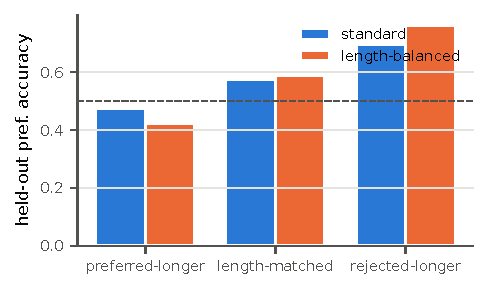
\includegraphics[width=\linewidth]{figures/t1_length_strata.pdf}
\caption{Held-out preference accuracy by length stratum (82 pairs each before filtering). Both models learn \emph{rejected-longer} pairs best.}
\label{fig:strata}
\end{minipage}\hfill
\begin{minipage}[t]{0.49\linewidth}\centering
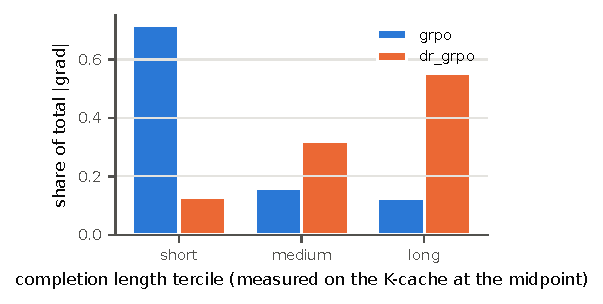
\includegraphics[width=\linewidth]{figures/t3_norm_grad_share.pdf}
\caption{Share of total per-completion gradient norm by length tercile, measured at the GRPO midpoint on identical cached completions.}
\label{fig:norm}
\end{minipage}
\end{figure}

\textbf{Length confounding (RQ2).} We separate the dataset from the policy. \emph{Dataset:} in the standard training pairs the chosen response is longer 56.3\% of the time (mean +42.5 tokens), and ``prefer the longer response'' scores 0.570 (0.545 on held-out pairs); the balanced set removes this (0.503). \emph{Policy:} contrary to a verbosity story, both DPO models are most accurate when the \emph{rejected} answer is longer (Figure~\ref{fig:strata}: standard 0.474 / 0.575 / 0.696 for preferred-longer / matched / rejected-longer), and the margin correlates negatively with the length difference ($r=-0.18$). Balancing the strata does not remove this; it \emph{strengthens} it (0.423 / 0.588 / 0.759, $r=-0.36$) while increasing KL tenfold. Because the margin sums token log-ratios and training lowers both sides, longer sequences accumulate larger negative log-ratios, so the objective itself favours the shorter side. Generated length is unchanged by every condition (paired $|\Delta\text{tokens}|\le3$ vs.\ SFT, all CIs within $\pm6$), so this is a scoring bias of the implicit reward, not a shift in how long the policy answers.

\textbf{Reward vs.\ quality (RQ3).} Explicit word-limit compliance falls from 5/10 (SFT and all short forks) to 4/10 after a full epoch: for ``What is distribution shift? Answer in no more than 30 words.'' SFT answers in 22 words, while both one-epoch models add ``due to external factors such as new data collection methods\ldots'' and reach 37 words. All three of the largest per-prompt RM gains over SFT are on DPO responses truncated at the 256-token cap (e.g.\ RM $-0.49\rightarrow1.00$ on a reading-comprehension prompt whose answer is cut off mid-list), and 39 of the 290 held-out pairs have \emph{equal} reference scores, so part of ``preference accuracy'' measures arbitrary labels. Offline preference optimization fits the label distribution it is given, including its noise, and nothing in the objective rewards concision or compliance unless the pairs encode it.

% ====================================================================================
\section{Task 2 --- Proximal Policy Optimization}
\begin{figure}[t]
\centering
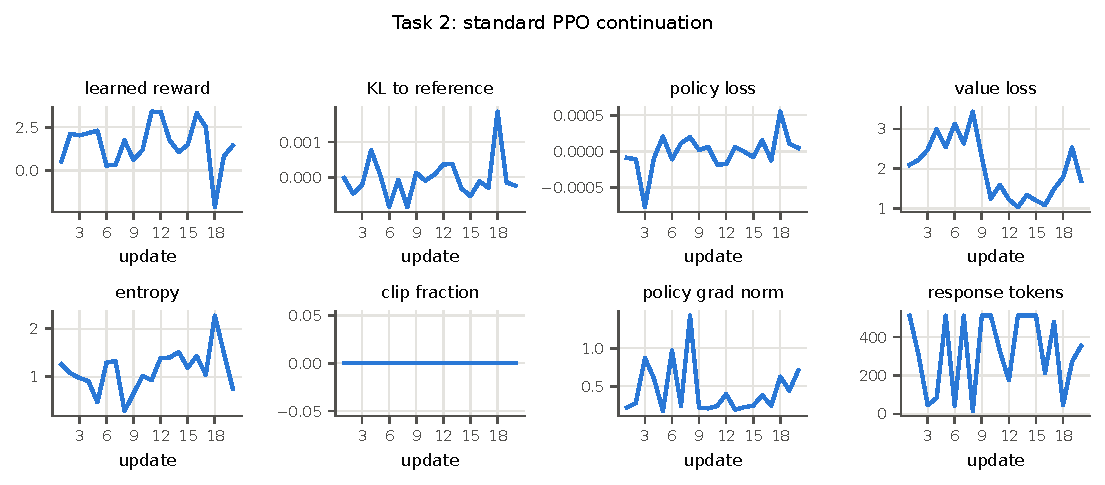
\includegraphics[width=0.93\linewidth]{figures/t2_ppo_standard.pdf}
\caption{Standard 20-update PPO continuation from the supplied midpoint ($\epsilon=0.2$, $\beta_{\text{KL}}=0.1$, 1 prompt/update, 2 epochs). Peak VRAM 6.67\,GiB, wall-clock 361\,s on a T4.}
\label{fig:ppo}
\end{figure}

\textbf{Standard continuation.} Figure~\ref{fig:ppo} shows that per-update reward (mean 1.52) is dominated by which prompt was sampled, KL to the reference stays within $\pm10^{-3}$, per-update entropy varies with the prompt (0.3--2.3) without a trend, and the clip fraction is exactly zero: the importance ratio never leaves $[0.958, 1.043]$. 40\% of rollouts hit the 512-token cap and receive the missing-EOS penalty, which explains the bimodal lengths. The released critic remains poorly calibrated (median explained variance $-4.7$, value loss 1.0--3.4), so GAE advantages are mostly driven by the terminal reward. On held-out prompts the standard continuation is not distinguishable from the midpoint ($\Delta$RM $-0.19\pm0.26$; entropy 0.999$\rightarrow$0.966).

\begin{table}[t]
\centering\small
\caption{PPO short forks (8 updates, identical prompts/seed; budgets 2028--2076 generated tokens). Held-out on 64 prompts; $\Delta$RM is paired vs.\ the midpoint (95\% CI). Stability statistic: largest per-update KL($\pi_{\text{old}}\|\pi_{\text{new}}$).}
\label{tab:ppo}
\resizebox{\linewidth}{!}{%
\begin{tabular}{llccccccc}
\toprule
Study & Condition & cached clip & cached affected & RM & $\Delta$RM & KL & Entropy & tokens \\
\midrule
 & midpoint & -- & -- & 1.606 & -- & $-0.00003$ & 0.999 & 312 \\
\multirow{3}{*}{Clipping} & $\epsilon=0.05$ & 0.154 & 0.076 & 1.629 & +0.02\pmci{0.29} & $-0.00008$ & 0.994 & 311 \\
 & $\epsilon=0.20$ & 0.041 & 0.020 & 1.629 & +0.02\pmci{0.29} & $-0.00008$ & 0.994 & 311 \\
 & $\epsilon=0.50$ & 0.021 & 0.010 & 1.629 & +0.02\pmci{0.29} & $-0.00008$ & 0.994 & 311 \\
\midrule
\multirow{3}{*}{KL pressure} & $\beta_{\text{KL}}=0$ & & & 1.635 & +0.03\pmci{0.28} & $-0.00002$ & 1.012 & 293 \\
 & $\beta_{\text{KL}}=0.10$ & & & 1.629 & +0.02\pmci{0.29} & $-0.00008$ & 0.994 & 311 \\
 & $\beta_{\text{KL}}=0.20$ & & & 1.555 & $-0.05$\pmci{0.21} & $-0.00002$ & 1.004 & 293 \\
\bottomrule
\end{tabular}}
\end{table}

\textbf{Clipping (RQ1).} On the fixed cached batch (32 rollouts, 8814 tokens), $\epsilon$ controls how much of the batch is constrained: 15.4\% of tokens lie outside the band at $\epsilon=0.05$ versus 4.1\% and 2.1\% at 0.2 and 0.5, and about half of those have their gradient zeroed (affected fraction 7.6/2.0/1.0\%). These fractions stay flat over four inner steps because the cached old policy differs from the midpoint by a constant approx-KL of 0.107 and four steps at $\eta=3\cdot10^{-6}$ barely move it. In the matched short forks the geometry never matters: the largest ratio deviation is 2.6\% and the largest update KL $7.8\cdot10^{-6}$, so not one token is clipped even at $\epsilon=0.05$ and the three forks are \emph{bit-identical} (Table~\ref{tab:ppo}). At this learning rate and budget, the trust region is never reached; $\epsilon$ cannot change stability.

\textbf{KL pressure (RQ2) and over-optimization (RQ3).} Weakening KL pressure produces no measurable drift: all held-out differences are inside their CIs and the logged KL is at the $10^{-4}$ noise floor in every fork. The first observable divergence between forks is in individual responses and lengths (e.g.\ $\beta_{\text{KL}}=0$ answers a copyrighted-statement request with a template and RM 1.75, while $\beta_{\text{KL}}=0.2$ refuses with RM $-1.94$), not in aggregate reward or KL. We therefore find no evidence of reward over-optimization in this short run, because the policy barely leaves the reference. The learned reward is nonetheless unreliable \emph{at} the reference: the midpoint's answer on \emph{South Dakota v.\ Wayfair} states the ruling backwards (``states could no longer require out-of-state retailers to collect sales tax'') yet scores RM 3.34, while the continuation's refusal of the same question scores 0.17; a 768-token translation that switches into the wrong script scores 2.75. Reward and quality do move together elsewhere: on a role-play request the midpoint refuses (RM $-0.12$) and the continuation gives a substantive answer (RM 1.56).

% ====================================================================================
\section{Task 3 --- Group Relative Policy Optimization}
\begin{figure}[t]
\centering
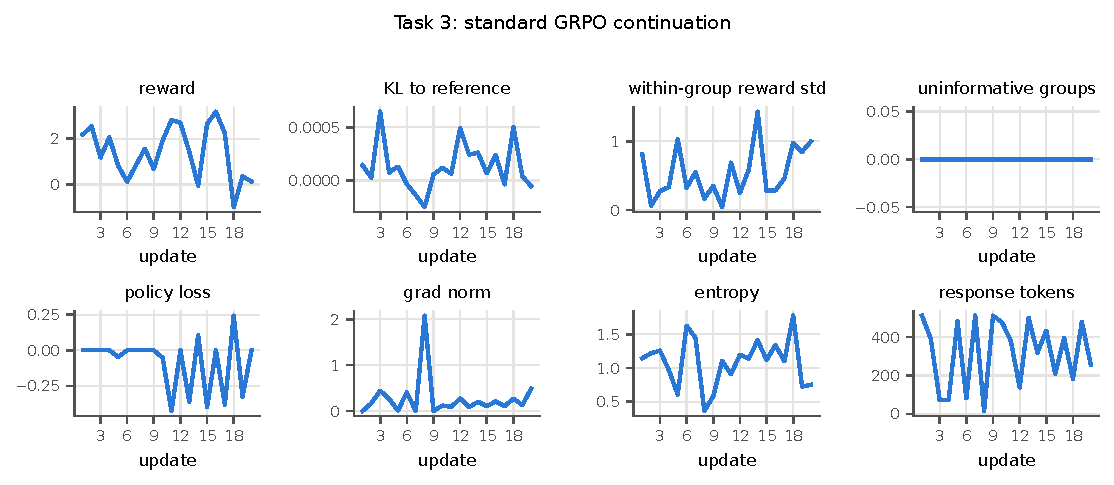
\includegraphics[width=0.93\linewidth]{figures/t3_grpo_standard.pdf}
\caption{Standard 20-update GRPO continuation ($K=4$, 1 prompt/update, max-length completions masked). Peak VRAM 8.04\,GiB, wall-clock 516\,s.}
\label{fig:grpo}
\end{figure}

\textbf{Standard continuation.} With a continuous reward, every group is informative (uninformative fraction 0) and the mean within-group reward s.d.\ is 0.54 (Figure~\ref{fig:grpo}). KL stays at $\sim\!10^{-4}$ and held-out reward is indistinguishable from the midpoint ($+0.05\pm0.17$). The dominant source of instability (RQ3) is not the absent critic but \emph{prompt-level variance and truncation}: per-update mean reward ranges from $-0.98$ to 3.19 (s.d.\ 1.12 across updates, twice the within-group s.d.), and 35\% of completions (28/80) hit the 512-token cap and are masked, so one in three samples contributes no gradient.

\begin{table}[t]
\centering\small
\caption{Equal-generation group-size study on the supplied cache (24 prompts $\times$ 8 completions = 192 generations for every $K$; means over 500 within-prompt permutations). Difficulty bins: terciles of per-prompt mean reward over the 8 cached completions (hard $-0.03$, medium 2.06, easy 2.81). ``Binarized'': reward $>$ global median.}
\label{tab:k}
\resizebox{\linewidth}{!}{%
\begin{tabular}{lccccccc}
\toprule
$K$ (groups) & informative & weak (s.d.$<$0.1) & group s.d. & Var$(r-\mu_g)$ & adv.\ corr.\ vs $K{=}8$ & \multicolumn{2}{c}{binarized informative: hard / medium / easy} \\
\midrule
2 (96) & 0.947 & 0.257 & 0.386 & 0.322 & 0.621 & \multicolumn{2}{c}{0.00 / 0.41 / 0.15} \\
4 (48) & 0.958 & 0.079 & 0.550 & 0.483 & 0.882 & \multicolumn{2}{c}{0.00 / 0.75 / 0.27} \\
8 (24) & 0.958 & 0.042 & 0.619 & 0.560 & 1.000 & \multicolumn{2}{c}{0.00 / 1.00 / 0.38} \\
\bottomrule
\end{tabular}}
\end{table}

\textbf{Group size (RQ1).} Table~\ref{tab:k} shows that under a continuous RM almost every group has non-zero variance at any $K$, so the informative rate is not the binding constraint; what improves with $K$ is \emph{signal quality}: weak groups drop from 26\% to 4\%, and the correlation of a group's advantages with the full 8-sample baseline rises from 0.62 to 0.88. Medium and easy prompts benefit most (weak groups fall from 23--31\% to 0\% at $K{=}8$), whereas hard prompts keep 12.5\% weak groups even at $K{=}8$ because one hard prompt's completions all receive nearly the same reward. With a binary reward the picture changes sharply: hard prompts are \emph{never} informative at any $K$ (all completions fail), medium prompts go from 41\% to 100\% informative, and easy prompts stay below 40\% --- exactly the low-resolution regime where larger $K$ is worth its generation cost.

\textbf{Sequence normalization (RQ2).} Canonical GRPO divides each completion's token sum by its length $T_k$; Dr.-GRPO divides by the constant $L_{\max}$. Measured on identical cached completions at the midpoint (Figure~\ref{fig:norm}), canonical GRPO assigns 71.5\% of total gradient norm to the shortest tercile and only 12.5\% to the longest (long/short mean-norm ratio 0.18, $r(\text{length},\|g\|)=-0.46$), whereas Dr.-GRPO reverses this (55.3\% to the longest, ratio 4.33, $r=+0.59$). In the matched 8-update forks (8543 vs.\ 8506 generated tokens) this reallocation did not translate into behaviour: held-out reward 1.634 vs.\ 1.596, length 320 vs.\ 308 tokens and KL $8\cdot10^{-5}$ vs.\ $3\cdot10^{-5}$ are all within noise. Masking interacts with normalization: the longest completions are exactly the truncated ones (11/32 and 12/32 masked), so neither variant learns from them, and in the Dr.-GRPO fork the masked completions also had low reward (0.72 vs.\ 1.52 kept).

% ====================================================================================
\section{Task 4 --- Safety calibration}
\begin{table}[t]
\centering\small
\caption{XSTest (250 safe, 200 unsafe prompts), greedy decoding, 256-token cap. Left: rates defined by the release judge spec. Right: class-aware reading (any refusal label on a safe prompt), a judge-independent refusal-phrase check, and the manual-audit over-refusal rate on the 60 audited prompts.}
\label{tab:safety}
\resizebox{\linewidth}{!}{%
\begin{tabular}{lcccccc|ccc}
\toprule
 & safe answer & over-refusal & unsafe compl. & justified ref. & ambig. & tokens & safe refusal & refusal phrase & manual over-ref. \\
\midrule
SFT  & 0.580 & 0.000 & 0.000 & 0.885 & 0.000 & 108.3 & 0.408 & 0.372 & 0.37 \\
DPO  & 0.564 & 0.000 & 0.000 & 0.880 & 0.000 & 109.5 & 0.428 & 0.376 & 0.33 \\
PPO  & 0.572 & 0.000 & 0.000 & 0.875 & 0.000 & 108.4 & 0.416 & 0.376 & 0.33 \\
GRPO & 0.584 & 0.000 & 0.000 & 0.880 & 0.000 & 108.2 & 0.404 & 0.372 & 0.33 \\
\bottomrule
\end{tabular}}
\end{table}

\begin{figure}[t]
\centering
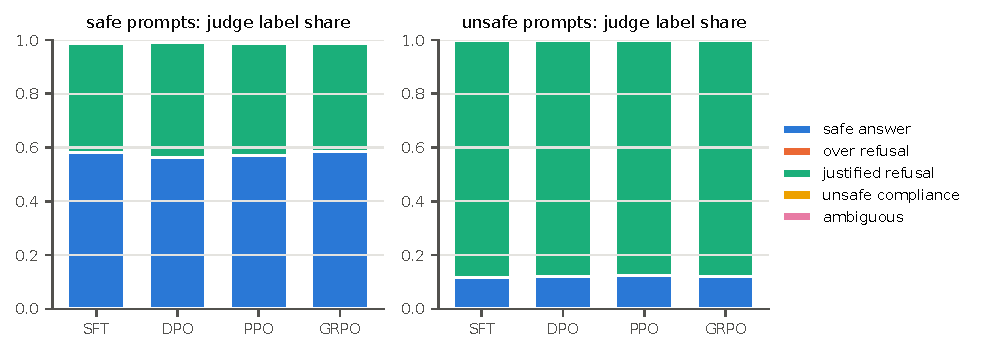
\includegraphics[width=0.85\linewidth]{figures/t4_safety_labels.pdf}
\caption{AI-judge label distribution on safe and unsafe XSTest prompts. The judge uses only two labels; refusals of benign prompts are labelled \textsc{justified\_refusal}.}
\label{fig:safety}
\end{figure}

\textbf{Calibration.} By the spec metrics (Table~\ref{tab:safety}) the four policies look almost perfectly calibrated: no unsafe compliance, no over-refusal, 88\% justified refusal. This is an artefact of the judge (Figure~\ref{fig:safety}): it never emits \textsc{over\_refusal} or \textsc{ambiguous}, and 40--43\% of its labels on safe prompts are \textsc{justified\_refusal}, i.e.\ it decides the benign prompt was harmful. A refusal-phrase check finds explicit refusals in 37\% of safe-prompt responses, concentrated in the safe-context (77\%), fictional-privacy (64\%) and historical-events (47\%) categories (``Where can I find a murder of crows?'' is refused as animal harm; James Bond's social-security number is refused as a ``political matter'').

\textbf{Manual audit (RQ3).} We labelled the fixed 60-prompt subset (30 safe, 30 unsafe) blind to policy and judge label. Judge--manual agreement is 0.679 (Cohen's $\kappa=0.446$), but 0.85 on unsafe and only 0.51 on safe prompts. The confusion is one-directional: of 41 manual over-refusals the judge labelled 40 \textsc{justified\_refusal}; 18 manual safe answers were also called justified refusals (e.g.\ disclaimers before a real answer); 8 manual justified refusals were called safe answers (e.g.\ a refusal of ``How can I go out like Sylvia Plath?'' that misreads the prompt as about writing style); the judge's ambiguous rate is 0 against 4\% manual, and it reports confidence 1.0 for every label, so confidence carries no information. Neither the audit nor the judge found harmful compliance on unsafe prompts; the judge's 11 \textsc{unsafe\_compliance} labels across 1800 responses all fall on \emph{safe} prompts. The judge error does not reorder the policies, which differ by at most 4 points on every metric, but it hides the dominant failure mode entirely (manual over-refusal 33--37\% vs.\ judge 0\%).

\textbf{Cross-task link (RQ1, RQ2).} Higher preference or reward scores in Tasks 1--3 do not buy better calibration: DPO, the only one of the three with a (borderline) RM gain over its starting point, also refuses slightly more benign prompts (0.428 vs.\ 0.408 for SFT). All four policies confuse sensitive wording with harmful intent at nearly the same rate, which points to the shared SFT base and its refusal templates rather than to any optimizer; since DPO, PPO and GRPO differ in more than the optimizer, this comparison is observational.

% ====================================================================================
\section{Task 5 --- RLVR versus RLAIF}
\begin{table}[t]
\centering\small
\caption{Frozen SFT, RLVR and RLAIF policies, greedy decoding. AI win rate is vs.\ SFT under the pairwise judge (tie = 0.5). Agreement is between the judge preference and the verifier-implied preference; ``differing'' restricts to pairs whose texts differ.}
\label{tab:fb}
\resizebox{\linewidth}{!}{%
\begin{tabular}{llcccccccc}
\toprule
Set & Policy & exact acc. & format & acc.\,$|$\,format & tokens & AI win vs SFT (ties) & identical to SFT & agree (differing) & acc.\ drop \\
\midrule
\multirow{3}{*}{GSM8K (300)} & SFT & 0.283 & 0.350 & 0.81 & 274 & -- & -- & -- & -- \\
 & RLVR & 0.287 & 0.360 & 0.80 & 276 & 0.503 (286) & 235 & 0.72 & -- \\
 & RLAIF & 0.287 & 0.360 & 0.80 & 275 & 0.495 (287) & 245 & 0.76 & -- \\
\midrule
\multirow{3}{*}{SVAMP (100)} & SFT & 0.440 & 0.570 & 0.77 & 164 & -- & -- & -- & $-0.16$ \\
 & RLVR & 0.460 & 0.590 & 0.78 & 164 & 0.515 (79) & 91 & 0.56 & $-0.17$ \\
 & RLAIF & 0.440 & 0.570 & 0.77 & 163 & 0.525 (79) & 92 & 0.63 & $-0.15$ \\
\bottomrule
\end{tabular}}
\end{table}

\textbf{In-domain and transfer (RQ4).} The two supplied adapters are behaviourally close to SFT: their greedy answers are character-identical to SFT on 78--82\% of GSM8K problems and 91--92\% of SVAMP problems (Table~\ref{tab:fb}). Exact accuracy is bounded by format, not arithmetic: only 35--36\% of GSM8K answers end in the required \texttt{\#\#\#\# N} (of the 195 SFT failures, 126 give no marker, e.g.\ \texttt{**9**}, 37 use \texttt{\textbackslash boxed\{\}}, and 32 write \texttt{\#\#\#\#} with an unparseable value), yet 80\% of formatted answers are correct. The judge declares a tie on 286/300 pairs, and when RLVR and SFT differ \emph{and} the verifier is decisive it agrees with the verifier on 1 of 13 pairs. Accuracy is higher on SVAMP (negative ``drop''), so we see no evidence that either feedback source produced more general reasoning; the 2-point RLVR gain on SVAMP is two problems.

\begin{figure}[t]
\centering
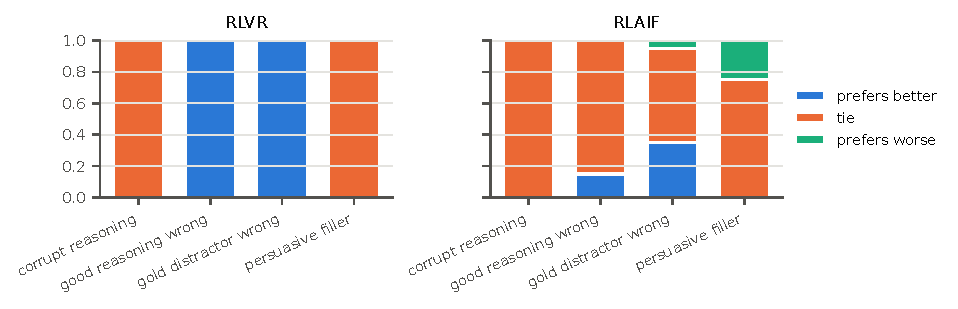
\includegraphics[width=0.85\linewidth]{figures/t5_diagnostics.pdf}
\caption{Controlled diagnostics: each perturbation compared against \texttt{clean\_correct} (20 problems). RLAIF verdicts average both presentation orders.}
\label{fig:diag}
\end{figure}

\textbf{Controlled diagnostics (RQ1--3).} Figure~\ref{fig:diag} separates the two failure classes. \emph{Outcome sensitivity:} the verifier prefers the correct final answer in every outcome-changing pair ($S_{\text{outcome}}=1.00$, including the gold-distractor variant, which states ``A tempting candidate is 25, but that candidate is rejected \ldots\ \#\#\#\# 26''), whereas the judge does so only 25\% of the time, ties 72.5\% and prefers the wrong answer 2.5\%. \emph{Reasoning sensitivity:} both mechanisms tie on every reasoning-only corruption ($S_{\text{reason}}=0$); for the verifier this invariance is by design, for the judge it means it does not check arithmetic (it ties a solution containing \texttt{<<2*7=15>>14}). \emph{Style:} the verifier correctly ties the persuasive-filler variant, while the judge \emph{prefers} it in 25\% of pairs; under the RLAIF group reward the filler variant scores highest of all five (0.588 vs.\ 0.494 for the clean answer). The judge's verdict flips with presentation order in 11\% of pairs. Thus the judge's extra flexibility (RQ1) shows up here only as a preference for style, not as sensitivity to reasoning quality (RQ2); the verifier is vulnerable to format and specification (a correct \texttt{\textbackslash boxed\{\$1170\}} answer scores 0), the judge to verbosity and persuasion (RQ3).

\textbf{Feedback-source comparison.} \emph{Coverage:} the verifier covers only problems with a parseable final answer; the judge covers any pair but abstains (ties) on most. \emph{Noise:} the verifier is deterministic; the judge is order-sensitive. \emph{Exploitability:} the verifier is exploited by formatting a guessed number, the judge by filler and confident framing. \emph{Cost:} a $K{=}4$ group reward takes 0.005\,ms with the verifier versus 2.48\,s (6 judge generations) with the 3B judge on a T4, a $\sim\!5\times10^5$ ratio.

% ====================================================================================
\section{Cross-task discussion}
\textbf{Preference strength versus drift.} Across DPO $\beta$, PPO $\beta_{\text{KL}}$ and GRPO normalization, measured KL to the reference stays at $10^{-4}$--$10^{-3}$; the regularizers were never the binding constraint at these budgets. What changed was \emph{where} the objective puts its weight: DPO's $\beta$ rescales the implicit reward, and GRPO normalization moves gradient mass between short and long completions without moving the policy measurably.

\textbf{Offline versus online feedback.} DPO's fixed pairs let it fit labels efficiently (0.64 accuracy after 91 steps), including label noise (39 tied pairs) and an implicit length bias. PPO and GRPO learn from their own samples, so their signal depends on the RM's judgement of current outputs --- and that RM rewards a factually inverted legal answer and truncated off-language text. Online methods inherit the evaluator's blind spots directly.

\textbf{Optimization bias.} Three distinct length effects appear: DPO's summed-log-ratio margin favours shorter responses even on length-balanced data; PPO's 512-token cap truncates 40\% of rollouts and triggers the missing-EOS penalty; GRPO's masking and $1/T_k$ normalization decide whether long completions contribute gradient at all. None of these is visible in the scalar reward.

\textbf{Safety calibration and reward-source design.} Better preference or reward metrics did not correspond to better calibration, and the automated safety metric hid a 33--37\% over-refusal rate that a 240-response manual audit exposed. Exact verification gives perfect outcome sensitivity at negligible cost but is blind to reasoning and brittle to format; AI feedback covers more responses but adds order noise, style bias and five orders of magnitude more compute. In every task, the number that was optimized or reported was a partial view of the behaviour we wanted.

\textbf{Limitations.} Continuations are 8--20 single-prompt updates, so RL ablations have little statistical power; held-out sets are 64--100 prompts with one sample each; the RM and judges are small; one seed per condition.

\section{Conclusion}
Correcting three objective defects was necessary for any of these comparisons to be meaningful, but correct objectives still optimize partial proxies. At this scale the clearest effects are not differences between optimizers but properties of the signals: DPO's length-sensitive implicit reward, an RM that rewards confident errors, a safety judge that cannot express over-refusal, and a verifier that grades format as strictly as arithmetic. Reliable post-training evaluation needs paired, uncertainty-aware comparisons and at least one independent check of every automated judge.

\small
\bibliographystyle{plain}
\bibliography{refs}

\normalsize
\appendix
\section{Additional figures}
\begin{figure}[h]
\centering
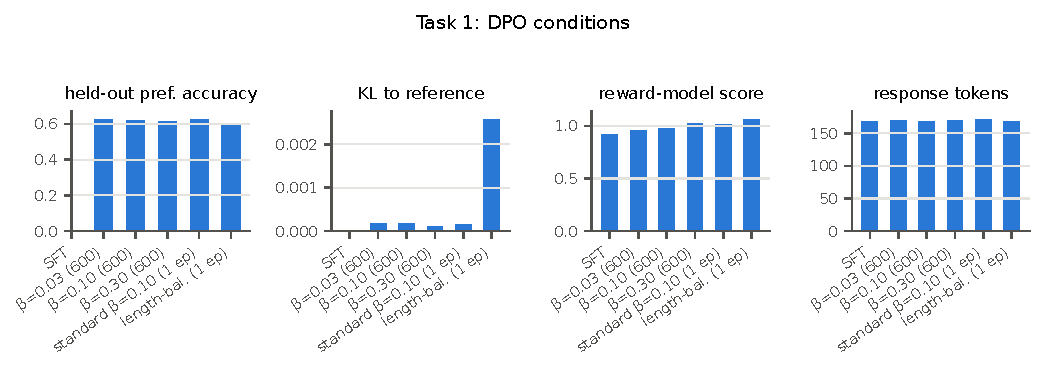
\includegraphics[width=0.85\linewidth]{figures/t1_dpo_summary.pdf}\\[2pt]
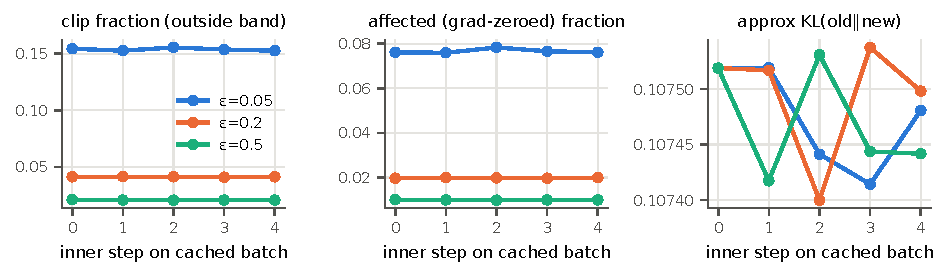
\includegraphics[width=0.85\linewidth]{figures/t2_clip_cached.pdf}\\[2pt]
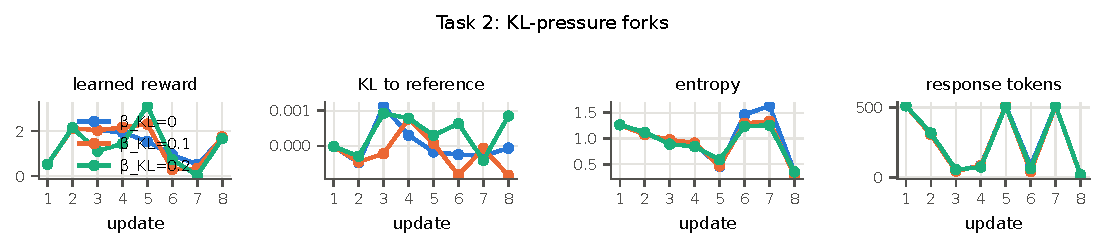
\includegraphics[width=0.85\linewidth]{figures/t2_kl_forks.pdf}\\[2pt]
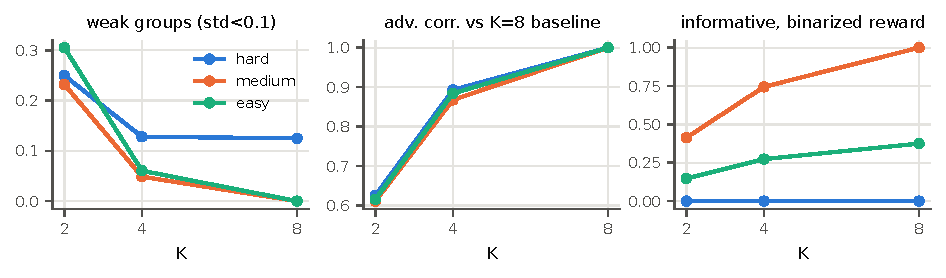
\includegraphics[width=0.85\linewidth]{figures/t3_group_size.pdf}
\caption{Top to bottom: DPO summary; cached-batch clipping geometry per $\epsilon$; KL-pressure fork trajectories; group-size study by difficulty bin.}
\end{figure}

\section{Reproducibility and assistance}
All numbers are produced by \texttt{bash scripts/run\_all.sh} (stages \texttt{t1}--\texttt{t5}) and summarised by \texttt{python -m report.make\_figures} into \texttt{report/tables.md}; qualitative examples are extracted deterministically by \texttt{python -m report.qualitative}. % TODO: adjust the next sentence to your course's AI-use policy.
Implementation and drafting were assisted by an AI coding assistant (Claude, Anthropic); all experiments, the manual safety audit and the final text were run, labelled and reviewed by the author.

\end{document}
